\section{1184006 - Murnia Lestari}
\subsection{Teori}
\begin{enumerate}

	\item Definisi Kecerdasan Buatan
	\hfill\break
	Kecerdasan Buatan atau Artifical Inteligence yang terdiri dari kata cerdas dan buatan. Cerdas artiya cepat dan tepat.  Sedangkan buatan artinya sesuatu yang sengaja dibuat dengan tujuan tertentu. Jadi kecerdasan buatan merupakan sebuah sistem yang disimulasikan dari kecerdasan yang dipunyai oleh manusia. Sehingga sistem ini akan melakukan pelkerjaan-pekerjaan yang umumnya dikerjakan oleh manusia secara cepat dan tepat seperti yang dilakukan oleh manusia. Point-point penting yang terdapat  dalam proses kecerdasan buatan adalah learning,reasoning dan self correction.

	\item Sejarah dan Perkembangan
	\hfill\break
Kecerdasan buatan bermula pada tahun 1940-an yang bermula dari kemunculan komputer. Kemudia pada tahun 1943 McMulloh dan Pitts pada tahun 1943 mempunyai usul untuk membuat model matematis yang bernama percepton dari neurin yang ada didalam otak. Pada tahun 1950 terbuatlah mesin turing yang mencoba menjawab “dapatkah computer berpikir” yang terdapat pada paper Alan Turing. Pada tahun 1955 akhir,Newell dan simon mengembangkan The Logic Theorist yaitu program kecerdasan buatan yang pertama. Pada tahun 1956 dari Massacuhetts Institute of Technology yaitu John McCharty yang dianggap sebagai bapak dari kecerdasan buatan atau AI menyelenggarakan konferensi untuk para ahli komputer dengan nama “ The Dartmouth summer research project on artifical intelligence. Pada tahun 1960-1970 muncullah “classical AI” yang merupakan diskusi mengenai bagaimana komputer dapat meniru dengan detail kemmapuan otak manusia. Dan pada tahun 1980 merupakan titik dimna kecerdasan buatan berkembang karena komputer dapat diperoleh dengan harga yag lebih murah.
	

	\item Kecerdasan buatan terbagi atas beberapa metode yaitu:
	\hfill\break
	Supervised learning,  Klasifikasi, Regresi,Unsupervised Learning, Dataset, Trainingset dan juga Testingset.
	\begin{itemize}
		\item Supervised Learning
		\hfill\break
	Supervised Learning	merupakan algoritma yang memiliki attribut tambahan seperti x dan y yang ingin diprediksi.
		\item Klasifikasi
		\hfill\break
		Klasifikasi merupakan sampel yang dimiliki oleh dua atau lebih kelas yang dikelompokkan yang disesuaikan berdasarkan ukuran kemiripan atau jarak yang melekat. 
		\item Regresi
		\hfill\break
Regresi	merupakan sebuah prediksi apabila hasil atau output yang diinginkan terdiri dari satu atau lebih variable contionous.
		\item Unsupervised Learning 
		\hfill\break
Unsupervised Learning  merupakan	algoritma yang tidak memiliki attribut tambahan yang akan diprediksi
		\item Data set
		\hfill\break
Data set	merupakan kondisi dimana hanya terdapat inputan data tanpa memiliki viariasi output yang sesuai
		\item Training Set
		\hfill\break
	Training Set	merupakan bagian dari data set yang digunakan untuk mempelajari beberapa properti		
		\item Testing Set
		\hfill\break
Testing Set	merupakan bagian data set yang digunakan untuk pengujian dari properti yang dipelajari
	\end{itemize}
\end{enumerate}
\subsection{Praktek}
\begin{enumerate}
	\item Instalasi Library scikit dari Anaconda, mencoba kompilasi dan uji coba ambil contoh kode dan lihat variabel explorer
	\hfill\break
	\begin{figure}[h]
		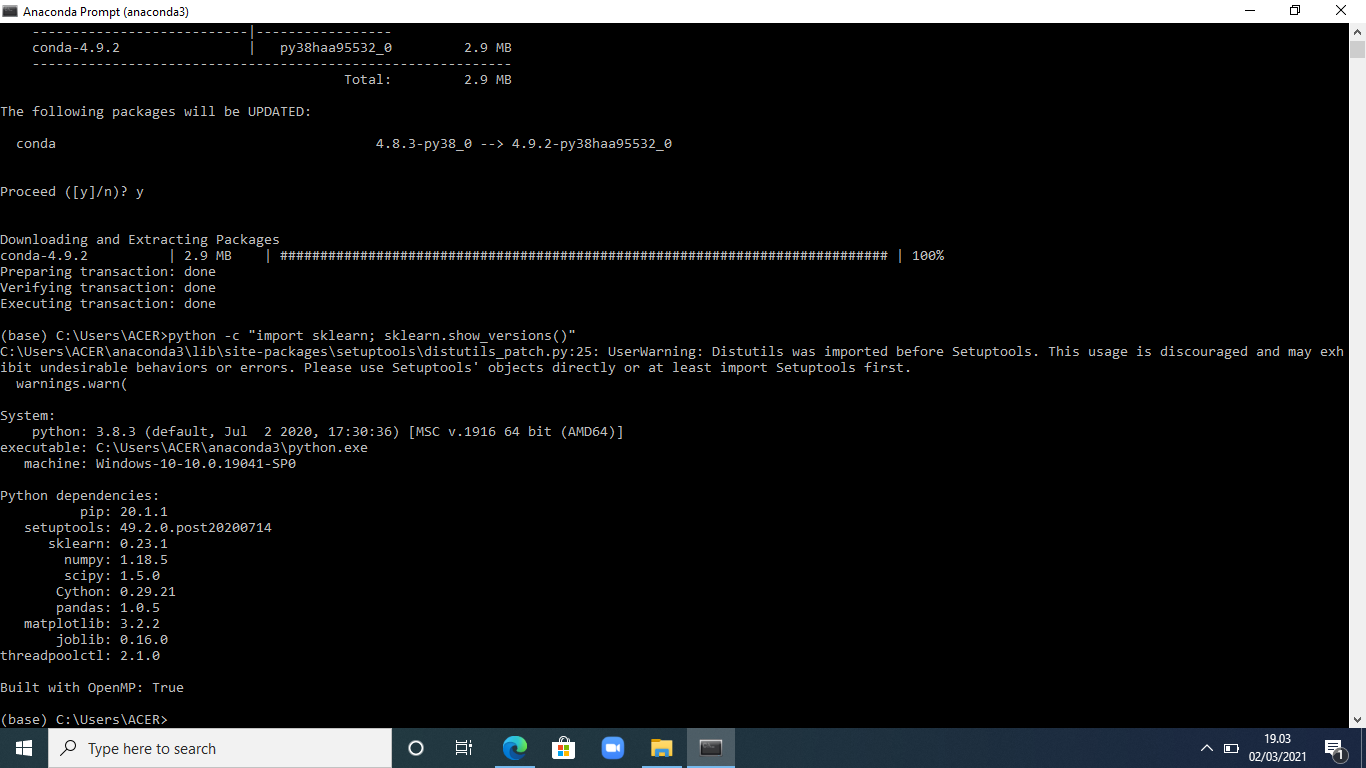
\includegraphics[width=10cm]{figures/1184006/chapter1/01.png}
		\centering
		\caption{Instalasi Library Scikit Learn}
	\end{figure}
	\begin{figure}[h]
		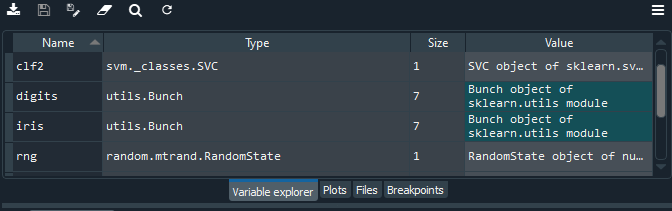
\includegraphics[width=10cm]{figures/1184006/chapter1/02.PNG}
		\centering
		\caption{Isi Variabel Explorer}
	\end{figure}
	\newpage\item Uji coba loading an example dataset
	\hfill\break
\lstinputlisting[firstline=7, lastline=16]{src/1184006/chapter1/tugas1.py}
\item Uji coba Learning dan predicting
	\hfill\break
	\lstinputlisting[firstline=17, lastline=32]{src/1184006/chapter1/tugas1.py}
\item Uji coba Model Persistence
	\hfill\break
	\lstinputlisting[firstline=35, lastline=63]{src/1184006/chapter1/tugas1.py}
	\item Uji coba Conventions
	\hfill\break
	\lstinputlisting[firstline=64, lastline=82]{src/1184006/chapter1/tugas1.py}
	\end{enumerate}
	\subsection{Penanganan Error}
\begin{enumerate}
	\item ScreenShoot Error
	\begin{figure}[h]
		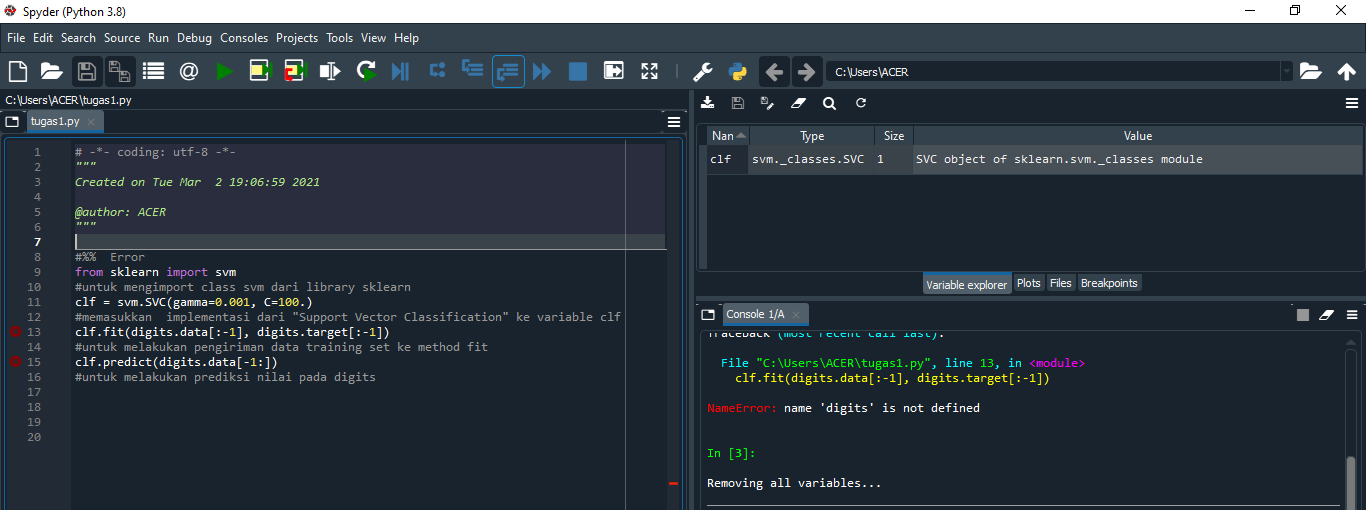
\includegraphics[width=10cm]{figures/1184006/chapter1/03.PNG}
		\centering
		\caption{Name Error}
	\end{figure}
	\newpage\item Tuliskan Kode Error dan Jenis Error
	\hfill\break
	\lstinputlisting[firstline=83, lastline=91]{src/1184006/chapter1/tugas1.py}
\hfill\break
	\item Cara Penangan Error
\hfill\break Tambahkan variabel digits agar kode program dapat terbaca
	\end{enumerate}
	\subsection{Bukti Tidak Plagiat}
\begin{figure}[h]
	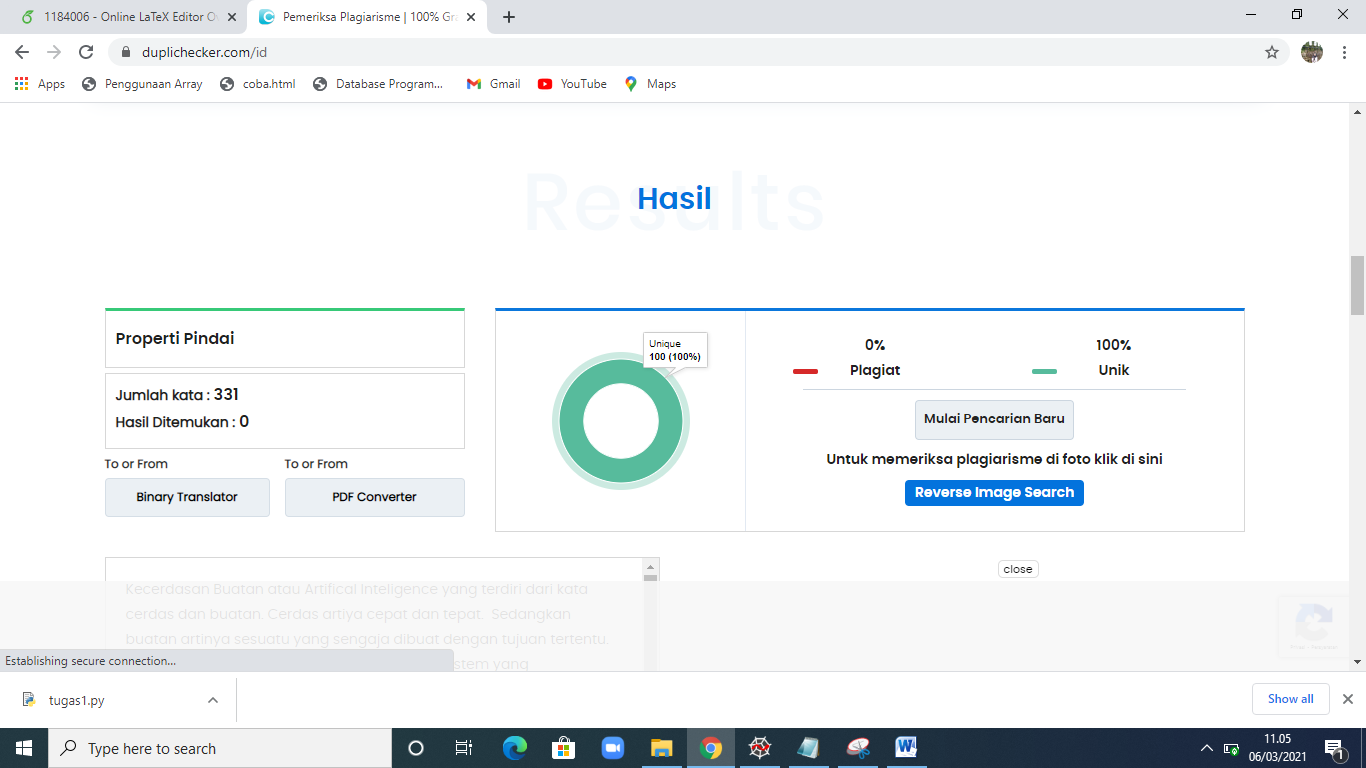
\includegraphics[width=10cm]{figures/1184006/chapter1/04.png}
	\centering
	\caption{Bukti Tidak Melakukan Plagiat Chapter 1}
\end{figure}